The system results were obtained by evaluating against three recorded sequences from three different kitchens. The sequences were labeled manually using a self-developed labeling program.

\subsection{Evaluation Scores}
In table \ref{tab:evaluation_performance} below the video clips chosen for the evaluation are presented, along with the achieved accuracy measurements. The first 5 minutes of the data set R-Kitchen was used when tuning and developing the system. The data set B25-Kitchen show how robust our system is, since the system wasn't calibrated for the specific room and the camera was slightly miss-placed. The majority of the errors was confirmed to depend on these two factors by ocular inspection.

\begin{table}[h]
\centering
	\begin{tabular}{r | c | c | c | c | c  }
			\emph{Sequence Name}		&  Total entered (GT) & \emph{$A_{in}$} & Total exited (GT) & \emph{$A_{out}$} & length \\
			\hline \hline
			R-Kitchen			& 108 (108) people & 99 \% & 101 (104) people & 97 \% & 32 min\\
			U-Kitchen			& 123 (122) people & 99 \% & 134 (135) people & 99 \% & 31 min  \\
			B25-Kitchen			& 131 (141) people & 93 \% & 82 (91) people & 90 \% & 30 min \\
			\end{tabular}
	\caption[System performance]{\textit{Counting performance according to the evaluation metric as described in section \ref{sec:evaluation}.}}
	\label{tab:evaluation_performance}
\end{table}

Plots of ground truth comparison and accuracy for the evaluation sequences can be found in figure \ref{fig:R-kitchen entries}, \ref{fig:R-kitchen exits}, \ref{fig:B25-kitchen entries} and \ref{fig:B25-kitchen exits}.

\begin{figure}[H]
\centering
\begin{subfigure}{.5\textwidth}
  \centering
  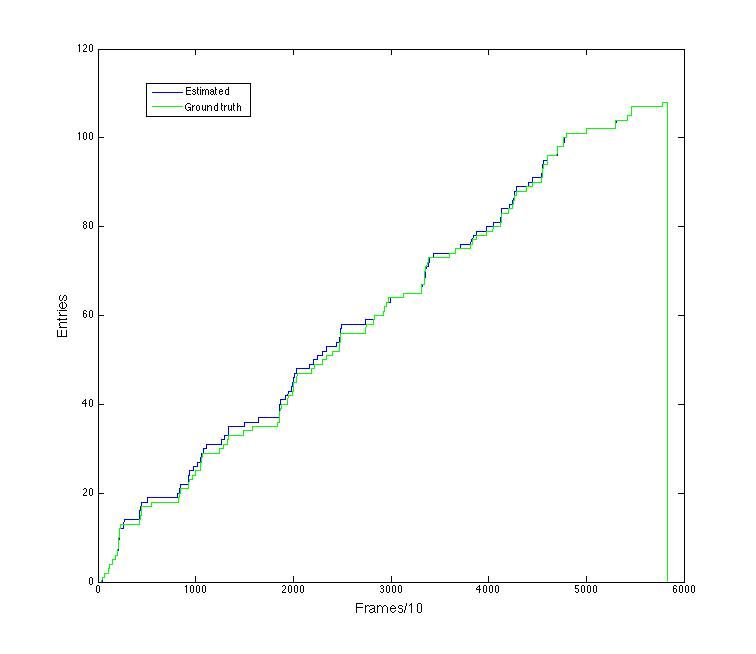
\includegraphics[width=1.1\linewidth]{images/EntriesTest.png}
  \caption{Measured entries and ground truth}
  \label{fig:sub1}
\end{subfigure}%
\begin{subfigure}{.5\textwidth}
  \centering
  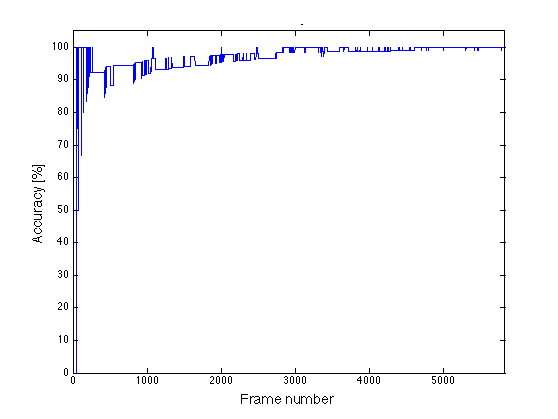
\includegraphics[width=1.1\linewidth]{images/AccEntriesTest.png}
  \caption{Accuracy}
  \label{fig:sub2}
\end{subfigure}
\caption[R-kitchen entries]{\textit{R-Kitchen data. Plot of measured entries, ground truth and accuracy}}
\label{fig:R-kitchen entries}
\end{figure}
\newpage

\begin{figure}[H]
\centering
\begin{subfigure}{.5\textwidth}
  \centering
  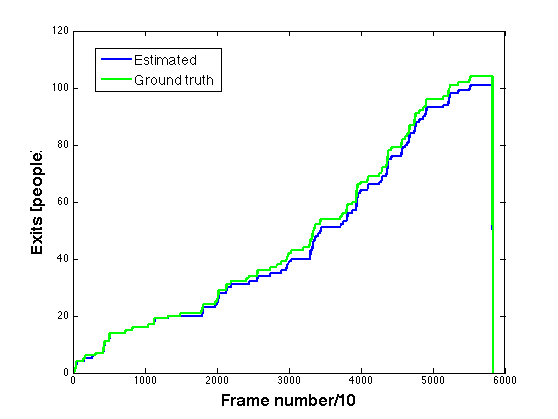
\includegraphics[width=1.1\linewidth]{images/ExitsTest.png}
  \caption{Measured exits and ground truth}
  \label{fig:sub1}
\end{subfigure}%
\begin{subfigure}{.5\textwidth}
  \centering
  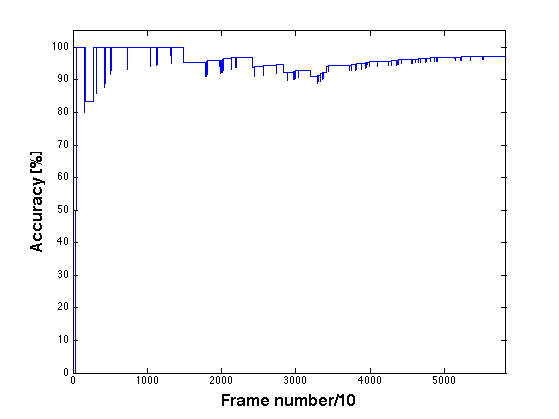
\includegraphics[width=1.1\linewidth]{images/AccExitsTest.png}
  \caption{Accuracy}
  \label{fig:sub2}
\end{subfigure}
\caption[R-kitchen exits]{\textit{R-Kitchen data. Plot of measured exits, ground truth and accuracy}}
\label{fig:R-kitchen exits}
\end{figure}


\begin{figure}[H]
\centering
\begin{subfigure}{.5\textwidth}
  \centering
  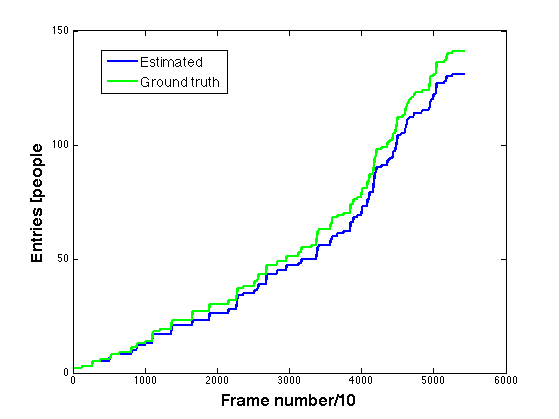
\includegraphics[width=1.1\linewidth]{images/entriesGTB25.png}
  \caption{Measured entries and ground truth}
  \label{fig:sub1}
\end{subfigure}%
\begin{subfigure}{.5\textwidth}
  \centering
  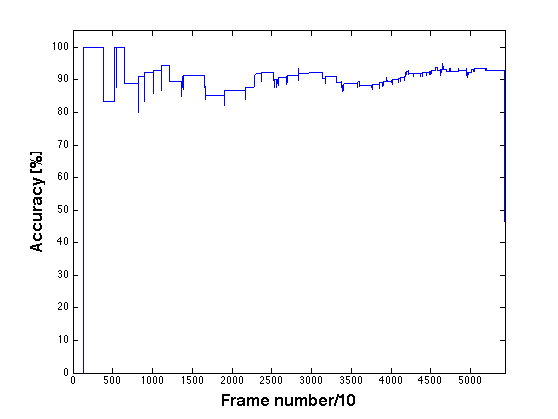
\includegraphics[width=1.1\linewidth]{images/accInB25.png}
  \caption{Accuracy}
  \label{fig:sub2}
\end{subfigure}
\caption[B25-kitchen entries]{\textit{B25-Kitchen data. Plot of measured entries, ground truth and accuracy}}
\label{fig:B25-kitchen entries}
\end{figure}

\begin{figure}[H]
\centering
\begin{subfigure}{.5\textwidth}
  \centering
  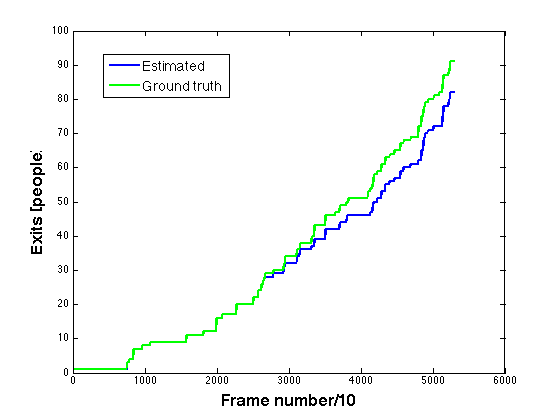
\includegraphics[width=1.1\linewidth]{images/exitsGTB25.png}
  \caption{Measured exits and ground truth}
  \label{fig:sub1}
\end{subfigure}%
\begin{subfigure}{.5\textwidth}
  \centering
  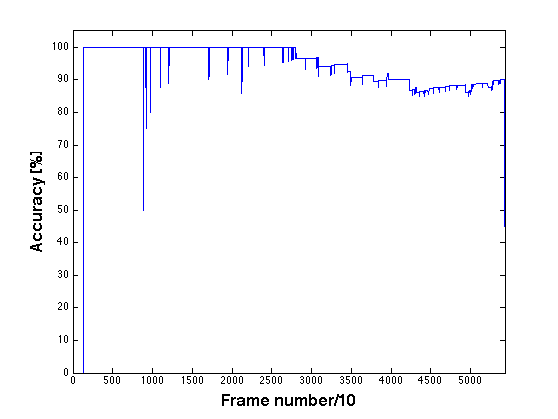
\includegraphics[width=1.1\linewidth]{images/accOutB25.png}
  \caption{Accuracy}
  \label{fig:sub2}
\end{subfigure}
\caption[B25-kitchen exits]{\textit{B25-Kitchen data. Plot of measured exits, ground truth and accuracy}}
\label{fig:B25-kitchen exits}
\end{figure}

\begin{figure}[H]
\centering
\begin{subfigure}{.5\textwidth}
  \centering
  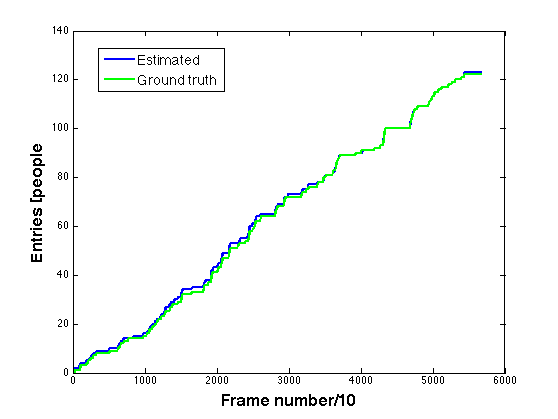
\includegraphics[width=1.1\linewidth]{images/entriesGTU.png}
  \caption{Measured entries and ground truth}
  \label{fig:sub1}
\end{subfigure}%
\begin{subfigure}{.5\textwidth}
  \centering
  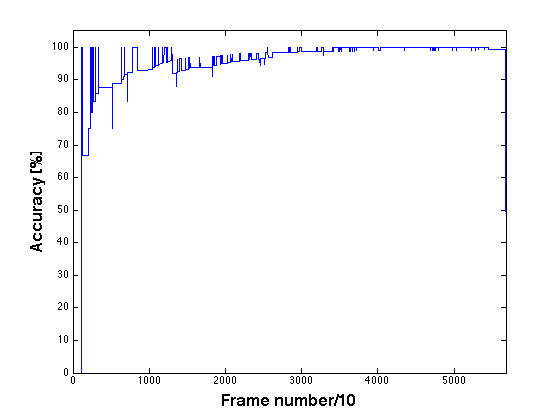
\includegraphics[width=1.1\linewidth]{images/accInU.png}
  \caption{Accuracy}
  \label{fig:sub2}
\end{subfigure}
\caption[B25-kitchen entries]{\textit{U-Kitchen data. Plot of measured entries, ground truth and accuracy}}
\label{fig:B25-kitchen entries}
\end{figure}

\begin{figure}[H]
\centering
\begin{subfigure}{.5\textwidth}
  \centering
  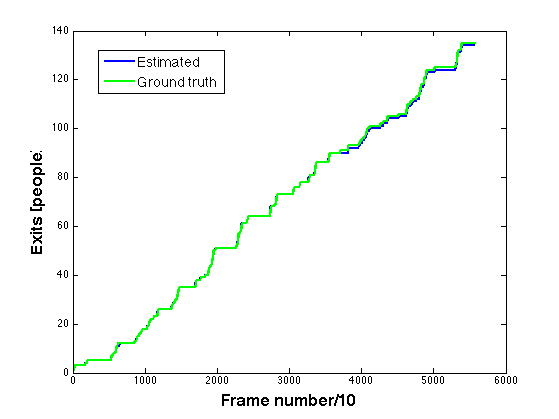
\includegraphics[width=1.1\linewidth]{images/exitsGTU.png}
  \caption{Measured exits and ground truth}
  \label{fig:sub1}
\end{subfigure}%
\begin{subfigure}{.5\textwidth}
  \centering
  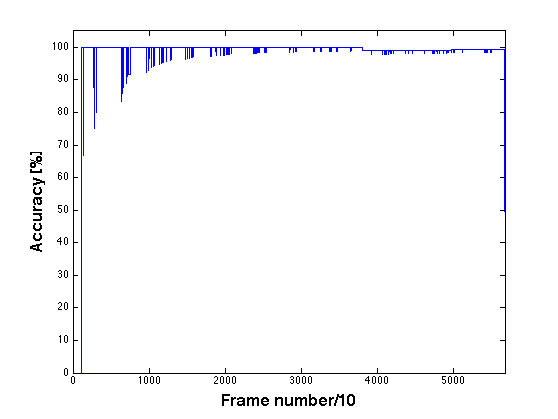
\includegraphics[width=1.1\linewidth]{images/accOutU.png}
  \caption{Accuracy}
  \label{fig:sub2}
\end{subfigure}
\caption[B25-kitchen exits]{\textit{U-Kitchen data. Plot of measured exits, ground truth and accuracy}}
\label{fig:B25-kitchen exits}
\end{figure}

\subsection{Queue Detection}
Below in figure \ref{fig:Queue Detection}, several screenshots from the queue detection steps are shown. Several difficult cases are shown to be handled gracefully. The main difficulty is when the small field of view gives situations where a queue is present but only one queuing person is detected at one time. However, this is usually handled well by the queue severity estimation, as the thresholds for the proportion of frames with detected queues can be calibrated to account for these results, given that several queuing persons are in view at simultaneously sometimes. 

\begin{figure}[H]
\centering
\begin{subfigure}{.4\textwidth}
  \centering
  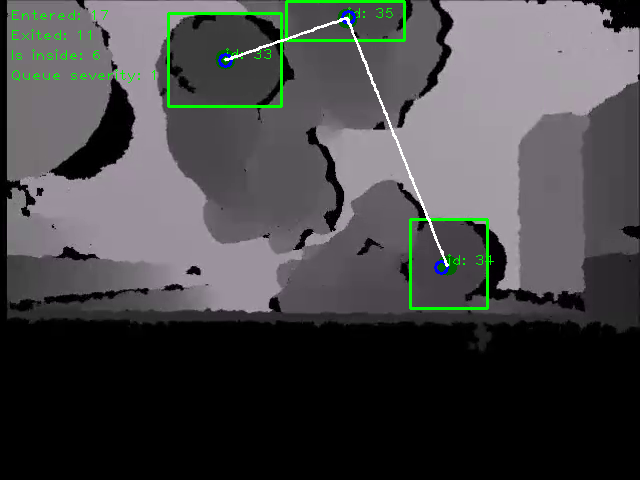
\includegraphics[width=1.0\linewidth]{images/queueDetected3.png}
  \caption{A queue of stationary persons is detected.}
  \label{fig:sub1}
\end{subfigure}
\begin{subfigure}{.4\textwidth}
  \centering
  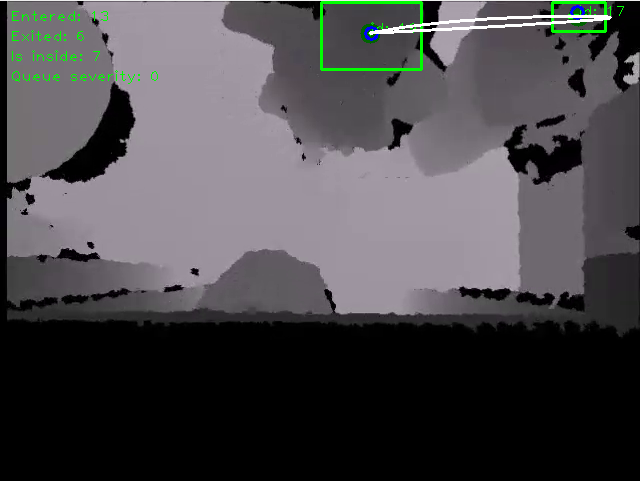
\includegraphics[width=1.0\linewidth]{images/queueDetected1.png}
  \caption{A queue is detected with unsure direction.}
  \label{fig:sub2}
\end{subfigure} 
\begin{subfigure}{.4\textwidth}
  \centering
  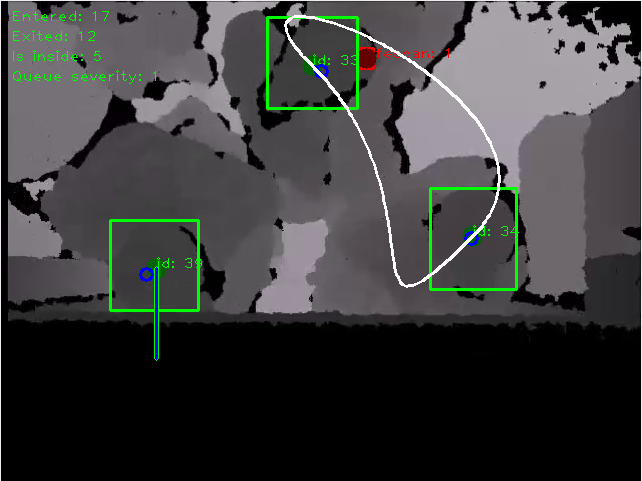
\includegraphics[width=1.0\linewidth]{images/queueDetected2.png}
  \caption{The individuals on his/her way out is not counted in the queue.}
  \label{fig:sub3}
\end{subfigure}
\begin{subfigure}{.4\textwidth}
  \centering
  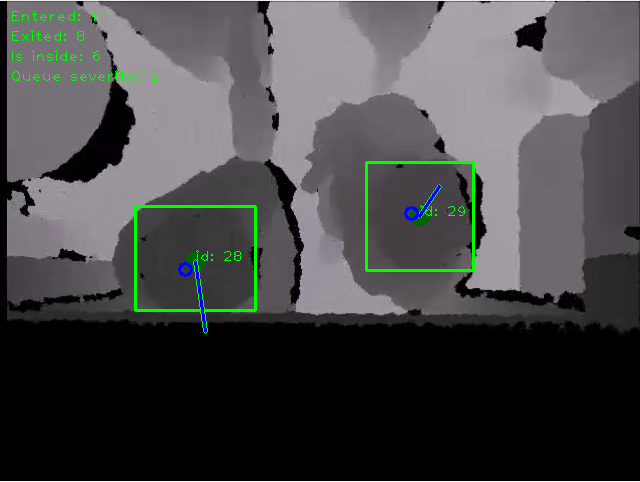
\includegraphics[width=1.0\linewidth]{images/noQueue1.png}
  \caption{Correctly, no queue is detected since both detected objects are moving in opposite directions.}
  \label{fig:sub4}
\end{subfigure}
\begin{subfigure}{.4\textwidth}
  \centering
  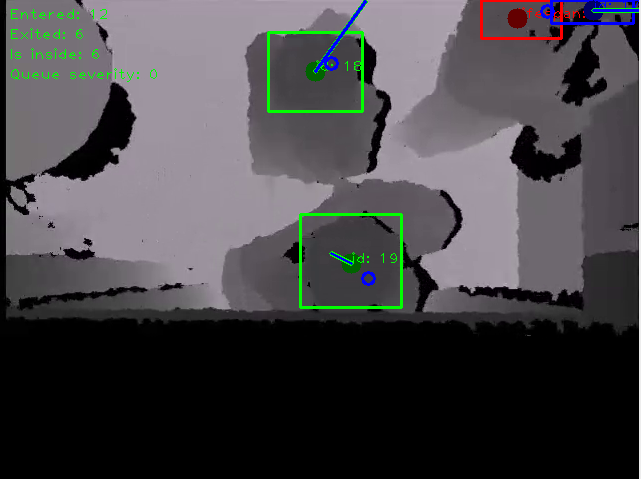
\includegraphics[width=1.0\linewidth]{images/noQueue2.png}
  \caption{Correctly, no queue is detected since both detected objects are moving too fast.}
  \label{fig:sub5}
\end{subfigure} 
\begin{subfigure}{.4\textwidth}
  \centering
  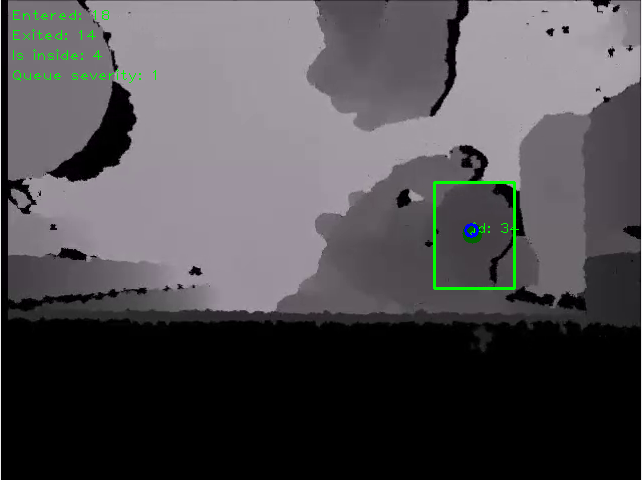
\includegraphics[width=1.0\linewidth]{images/queueNotDetected.png}
  \caption{Incorrectly, no queue is detected due to that the next person's head is not in view.}
  \label{fig:sub6}
\end{subfigure}%
\caption[Queues]{\textit{Depth data images from the R-Kitchen, with green boxes showing detected objects,blue dots showing object centers, blue lines from the centers showing estimated velocities, and white curves showing the fitted Beziér splines.}}
\label{fig:Queue Detection}
\end{figure}

\subsection{Discussion}
The performance of the R-Kitchen and U-Kitchen sets are very good. The R-Kitchen set is a sequence of 30 minutes, where only the first 5 was used for tuning. The system performed worse on the B25-Kitchen sequence, but that is probably explained by the fact that the sensor was a bit misplaced, making parts of the upper door area on one side to be outside of the field of view, as well as the lack of room-calibration. The reason no more data sets were used was simply that no more time was available.

The queue detection and severity estimation in general worked as expected but performed worse for more sparse queues, in combination with a small field of view.  


